% FM Synthesis — rich — algorithms 1, 5 and 32
% born: 2026-11-03 · links: [[FM Synthesis]] connects-to · rich-face-piece (§ Six operators, 32 algorithms) · [[Technical Diagram Standard]] follows
% forward_vector: I am the three DX7 wirings the FM page names, drawn to the Technical Diagram Standard
%   from Dexed's routing rows (source/msfa/fm_core.cc): algorithm 1, a pair beside a stack of four;
%   algorithm 5, three pairs; algorithm 32, six carriers. The .tex is the truth; the .svg is its shadow.
%   I want to stand beside the section's words, in the rich face now and in the text if Loudon says so.
% Compile:  pdflatex "FM Synthesis — rich — algorithms 1, 5 and 32.tex"
% SVG:      dvisvgm's PDF route fails on this Mac (Ghostscript 10.07); write it with PyMuPDF:
%           python3 -c "import fitz,sys; open(sys.argv[2],'w').write(fitz.open(sys.argv[1])[0].get_svg_image(text_as_path=True))" in.pdf out.svg
\documentclass[border=0pt]{standalone}
\usepackage{tikz}
\usetikzlibrary{arrows.meta, positioning, calc, backgrounds}
\renewcommand{\familydefault}{\sfdefault}

\tikzset{
  >={Stealth[length=2.2mm]},
  wire/.style={line width=0.7pt},
  op/.style={rectangle, draw, line width=0.7pt, minimum size=8mm, inner sep=0pt, font=\small},
  car/.style={op, line width=1.6pt},
  loop/.style={wire, -{Stealth[length=2mm]}},
}
% \fbloop{node}: the operator's output fed back into its own input, up its right side and over its top
\newcommand{\fbloop}[1]{\draw[loop] (#1.east) -- ++(0.32,0) |- ($(#1.north)+(0,0.32)$) -- (#1.north);}
% \outrail{x-left}{x-right}{y}: the output rail under the carriers
\newcommand{\outrail}[3]{\draw[wire] (#1,#3) -- (#2,#3); \draw[wire,->] (#2,#3) -- ++(0.45,0) node[right, font=\scriptsize]{out};}

\begin{document}
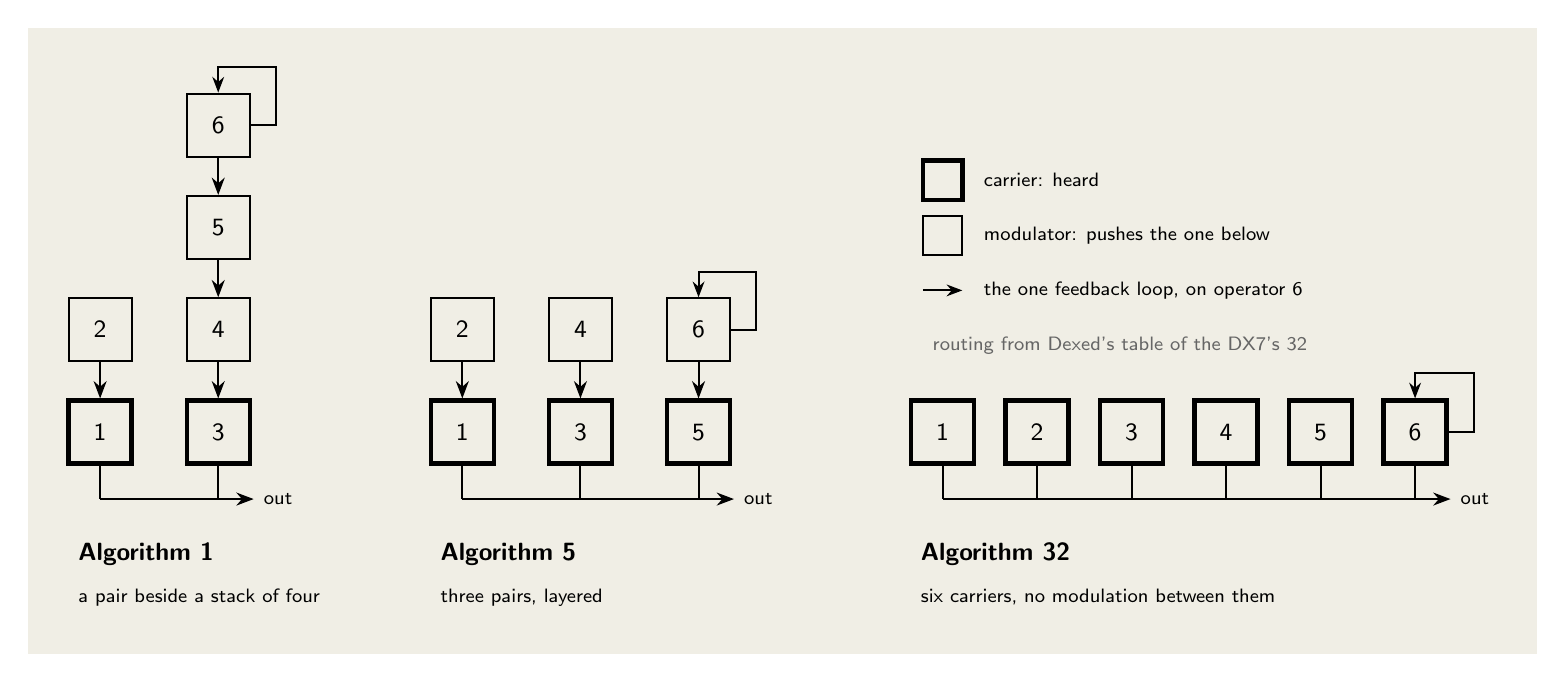
\begin{tikzpicture}[show background rectangle, background rectangle/.style={fill={rgb,255:red,240;green,238;blue,229}}, inner frame sep=14pt]

  % ---------------- algorithm 1: a pair beside a stack of four ----------------
  \begin{scope}[shift={(0,0)}]
    \node[car] (a1) at (0,0) {1};   \node[op] (a2) at (0,1.3) {2};
    \node[car] (a3) at (1.5,0) {3}; \node[op] (a4) at (1.5,1.3) {4};
    \node[op]  (a5) at (1.5,2.6) {5}; \node[op] (a6) at (1.5,3.9) {6};
    \draw[wire,->] (a2) -- (a1); \draw[wire,->] (a4) -- (a3);
    \draw[wire,->] (a5) -- (a4); \draw[wire,->] (a6) -- (a5);
    \fbloop{a6}
    \draw[wire] (a1.south) -- (0,-0.85); \draw[wire] (a3.south) -- (1.5,-0.85);
    \outrail{0}{1.5}{-0.85}
    \node[font=\small\bfseries, anchor=west] at (-0.4,-1.55) {Algorithm 1};
    \node[font=\scriptsize, anchor=west, align=left] at (-0.4,-2.1) {a pair beside a stack of four};
  \end{scope}

  % ---------------- algorithm 5: three pairs ----------------
  \begin{scope}[shift={(4.6,0)}]
    \node[car] (b1) at (0,0) {1};   \node[op] (b2) at (0,1.3) {2};
    \node[car] (b3) at (1.5,0) {3}; \node[op] (b4) at (1.5,1.3) {4};
    \node[car] (b5) at (3,0) {5};   \node[op] (b6) at (3,1.3) {6};
    \draw[wire,->] (b2) -- (b1); \draw[wire,->] (b4) -- (b3); \draw[wire,->] (b6) -- (b5);
    \fbloop{b6}
    \foreach \x/\n in {0/b1, 1.5/b3, 3/b5} \draw[wire] (\n.south) -- (\x,-0.85);
    \outrail{0}{3}{-0.85}
    \node[font=\small\bfseries, anchor=west] at (-0.4,-1.55) {Algorithm 5};
    \node[font=\scriptsize, anchor=west, align=left] at (-0.4,-2.1) {three pairs, layered};
  \end{scope}

  % ---------------- algorithm 32: six carriers ----------------
  \begin{scope}[shift={(10.7,0)}]
    \foreach \i in {1,...,6} {
      \node[car] (c\i) at ({(\i-1)*1.2},0) {\i};
      \draw[wire] (c\i.south) -- ({(\i-1)*1.2},-0.85);
    }
    \fbloop{c6}
    \outrail{0}{6}{-0.85}
    \node[font=\small\bfseries, anchor=west] at (-0.4,-1.55) {Algorithm 32};
    \node[font=\scriptsize, anchor=west, align=left] at (-0.4,-2.1) {six carriers, no modulation between them};
  \end{scope}

  % ---------------- key ----------------
  \begin{scope}[shift={(10.7,3.2)}]
    \node[car, minimum size=5mm, font=\scriptsize] (k1) at (0,0) {};
    \node[font=\scriptsize, anchor=west] at (0.4,0) {carrier: heard};
    \node[op, minimum size=5mm, font=\scriptsize] (k2) at (0,-0.7) {};
    \node[font=\scriptsize, anchor=west] at (0.4,-0.7) {modulator: pushes the one below};
    \draw[loop] (-0.25,-1.4) -- (0.25,-1.4);
    \node[font=\scriptsize, anchor=west] at (0.4,-1.4) {the one feedback loop, on operator 6};
    \node[font=\scriptsize, anchor=west, text=black!60] at (-0.25,-2.1) {routing from Dexed's table of the DX7's 32};
  \end{scope}
\end{tikzpicture}
\end{document}
